% Suggested topics:
% Triangle fixig, timeslices (different from DT), MCMC, moves, chosen topology

% TODO: mist er nog niet iets over het feit dat we MCMC kiezen, dat in ieder geval noemen
\begin{frame}
    \frametitle{Volume fixing}
    Split $Z$ into fixed volume contributions:
    \begin{equation}
        Z
        =
        \sum_{T_\ell} \frac{1}{N_2(T_\ell)!} e^{-\lambda N_2(T_\ell)}
        =
        \sum_{n = 0}^\infty \Omega(n) \frac{e^{-\lambda n}}{n!}
    \end{equation}
    It turns out that $\Omega(n) \sim n! 2^n$ \\
    Problem:
    \begin{itemize}
        \item $\lambda > \ln 2$: typical triangulation has a very small volume $\to$ cannot extract useful data
        \item $\lambda < \ln 2$: triangulation keeps growing $\to$ equilibrium cannot be reached
    \end{itemize}
    Solution: fix the number of triangles $N_2$
\end{frame}

\begin{frame}
    \frametitle{Volume fixing (2)}
    Possible solution: add a constraint term $\delta S = \epsilon \abs{N_2(T) - n}$ \\
    Issues:
    \begin{itemize}
        \item Introduces an extra parameter $\epsilon$
        \item Results in more rejections
    \end{itemize}
    Alternative: use update rules that preserve $N_2$ \\
    Futher advantage: distribution becomes uniform
\end{frame}

\begin{frame}
    \frametitle{Update Rules}
    \begin{figure}
        \centering
        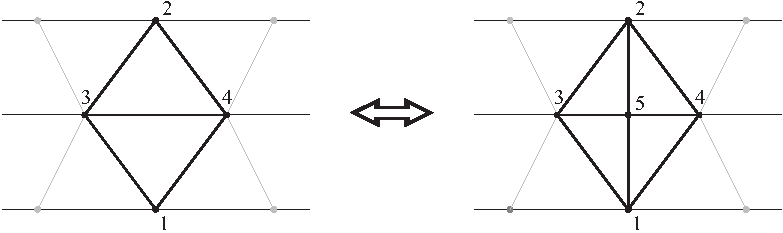
\includegraphics[width=0.6\linewidth]{shard_move}
    \end{figure}
    \begin{itemize}
        \item Take a "shard" and insert it somewhere else
        \item Requires order 4 vertex (keep a list)
        \item Detailed balance: Yes
        \item Ergodic: No
    \end{itemize}

\end{frame}

\begin{frame}
    \frametitle{Update Rules (2)}
    \begin{figure}
        \centering
        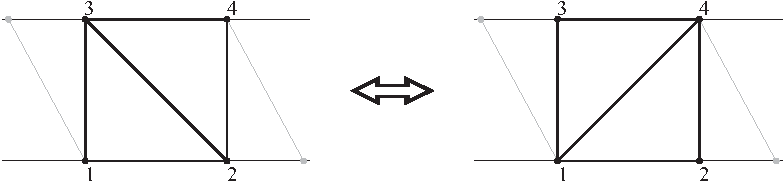
\includegraphics[width=0.6\linewidth]{flip_move}
    \end{figure}
    \begin{itemize}
        \item Uniformly choose a triangle and flip it
        \item Requires oppositely oriented neighbour
        \item Detailed balance: Yes, with rejections
        \item Ergodic: Yes
    \end{itemize}
    Two different moves: introduce move ratio $r = p(\text{shard move})$
\end{frame}